\documentclass[12pt,a4paper]{article}
\usepackage[utf8]{inputenc}
\usepackage[margin=2.5cm]{geometry}
\usepackage[super]{natbib}
\usepackage[breaklinks]{hyperref}
\usepackage[noabbrev]{cleveref}
\usepackage[bottom]{footmisc}
\usepackage{enumitem}
\usepackage{ragged2e}
\usepackage{multirow}
\usepackage[
    left = `,%
    right = ',%
    leftsub = ``,%
    rightsub = "%
]{dirtytalk}
\usepackage{graphicx}
\usepackage{wrapfig}
\usepackage{caption}
\usepackage{subcaption}
\usepackage[font=small,labelfont=bf]{caption}
\usepackage{booktabs}

%
% Commands
%

\def\code#1{\texttt{#1}}

%
% Formatting
%

\linespread{1.6}

\bibliographystyle{plainnat}
% \setcitestyle{numbers}
\setcitestyle{square}

\setlength{\abovedisplayskip}{5pt}
\setlength{\skip\footins}{7pt}

%
% Title formatting
%

\title{
    % \vspace{100pt}
    \textsc{\Large Trends in Accident \& Emergency Waiting Times \\
    from NHS UK }
}
    
\date{May 2022}
\author{Jakub Malý and Julia Miklas}

\begin{document}

%
% Title page
%

\maketitle
\thispagestyle{empty}

%
% Table of Contents
%

\vspace{5em}
\renewcommand{\baselinestretch}{1.4}\normalsize
\tableofcontents
\renewcommand{\baselinestretch}{1.6}\normalsize

\renewcommand{\thefootnote}{\Roman{footnote}}

\newpage
\pagenumbering{arabic}
\setcounter{page}{1}

%
% Text body
%

\section{Introduction}

NHS Scotland's accident and emergency departments (A\&Es) have a 4-hour wait standard (more than 95\% of patients should be admitted, discharged, or transferred within 4 hours from arrival). We look at the NHS statistics for A\&E patients between 2007 and 2021 and visualise trends within the data. We concentrate on how the NHS board, population size, and seasonality affect the compliance to the standard. 

Our findings show that the percentage of patients seen within 4 hours (henceforth referred to as the compliance percentage) has been on a long-term decreasing trend (0,205\% per year), with emergency departments having the steepest decline (0,574\% per year). Furthermore we identified that some of the possible factors causing this drop in compliance are winter pressures, hospital infrastructure not scaled to population needs and increase in unnecessary or misdirected attendances. 

Since we cannot predict how trends will evolve after the pandemic, all of our long-term analyses were done on data before March 2020. This allows us to isolate the underlying trends and better identify issues that were present before the pandemic. However, we have also qualitatively explored how the compliance of hospitals changed during the COVID-19 pandemic.

\subsection{Context and motivation} 

The specific percentage for the 4 hour NHS wait care standard was only specified in 2004. It was originally set to 98\% by the Labour government at the time but due to coalition opposing it on the premise that the target was not clinically justifiable it was brought down to 95\% in 2010.\cite{the_guardian_2013} In May 2021, NHS England announced that the 95\% standard would be replaced by a new bundle of then standards but it is yet unclear if this new policy will be expanded to the rest of the UK.

Evidently, wait time is an issue that has been discussed in depth and there are an increasing amount of studies on the matter. Analysing healthcare data is beneficial, since it is the primary way of identifying issues within the system. Examining wait times is especially vital to ensuring that people have access to high-quality healthcare, since prolonged waits can have impacts from financial losses to generating excess mortalities.\cite{iacobucci_2021}

\subsection{Previous work} 

Given the scope and importance of this issue, several independent organisations have already conducted analyses on NHS performance:
\begin{itemize} 
    \item The King's Fund utilises more granular time data, and tries to identify the causes for the decline of compliance for NHS England. It found that a new five-year funding deal would allow for performance to increase but not enough to recover up to full compliance without having to compromise the quality of their services, especially when taking into consideration staffing shortages.\cite{the_kings_fund_2020}
    \item The Nuffield Trust explores breaches of the four hour target in the context of a possible review of NHS access standards. It found that not only there is a constantly increasing number of patients waiting  in the waiting room but also an increase in so called "trolley waits", the wait between being seen and being admitted due to lack of available beds.\cite{the_nuffield_trust_2022}
    \item A publication by George Stoye observes how setting a wait time target has actual impacts patient care, on average increasing cost per patient but decreasing mortality and looks into the repercussions of changing wait time standards.\cite{stoye_2020}
\end{itemize}

\subsection{Our goals} 

\begin{itemize}
    \item Show that hospitals do not comply with the 4-hour standard.
    \item Show the yearly and long-term trends of the compliance rates.
    \item Discuss how the COVID-19 pandemic has affected the aforementioned trends.
    \item Show correlated demographics such as location and population and look for correlations with the waiting times.
\end{itemize}

\newpage

\section{Data}

Here, we give an overview of the data sets used, how they were obtained, and a short summary of how we used the data in our analysis. For more details (including exact dates of access), please visit the code repository.\cite{code}

\subsection{NHS data}

The main data set with hospital statistics was downloaded from the NHS Scotland website and is a publicly available data set.\cite{nhs_data} It is a monthly aggregate on a per-hospital basis, and includes the number of patients with wait times under 4 hours, over 8 hours and over 12 hours, as well as the type of discharge (residence, admitted, transferred, other and unknown). The data also labels each hospital with type of injury it treats (Emergency Department or Minor Injury Unit / Other) and the NHS Board it belongs to. To better read and visualise the data set the following operations were carried out on it:
\begin{itemize}
    \item The date column was reformatted into a year and (numeric) month columns, as well as a \code{year\_month} string that can be ordered correctly.
    \item Episodic data was dropped, since it was a less complete version of the aggregate data.
    \item The wait time data was converted into bins of 0--4, 4--8, 8--12 and 12+ hours waited: 8--12 bin was obtained by subtracting 12+ from 8+ data, and the 4--8 bin was obtained by subtracting all other bins from the total).
    \item A fractional compliance value was calculated as a ratio of the \code{under4h} and \code{total} data columns, as well as a boolean value whether this meets or exceeds the 95\% standard. 
\end{itemize}
The final processed data set contains 15471 entries spanning from July 2007 to December 2021.

\subsection{Geographical data}

The geographical borders data set was downloaded from Improvement Services' SpatialHub and under the UK Open Government Licence is free for use.\cite{geodata} The shapefile was converted using the \code{geopandas} Python package that uses the Geospatial Data Abstraction Library (GDAL). The geographical data included a polygon border for each council in Scotland, as well as which local authority the council belonged to. Polygons were aggregated via a shape union by local authority, and then further merged into NHS boards by manually defining authority-board pairs using the NHS website.\cite{nhs_boards} This allowed us to merge the data set with the NHS data by adding a polygon to each NHS board.

\subsection{Population data}

The population data was a part of a larger collection of data sets that were downloaded from the Scottish government's National Records of Scotland website.\cite{pop_data} The population data included a yearly population per council area per sex per age for years between 1998 and 2019. The data was grouped by year to obtain the total yearly population of each council area. The council area column included "Scotland" values which were dropped as we are interested in examining trends on a smaller scale. Councils were then mapped to NHS Boards using the same authority-board pairs as the geographical data.\cite{nhs_boards}

\section{Data analysis}

The main statistic of interest is the compliance (defined as the percentage of patients is seen within 4 hours), and whether it is above the 95\% standard. From Figure \ref{fig:fig1} we can see that the trend is on a general decline, both for emergency departments (EDs) and minor injury units (MIUs).

We used an Ordinary Least Squares (OLS) regression from Python's \code{statsmodels} package to calculate the fractional change in compliance for combined, ED-only, and MIU/Other-only hospitals. To mitigate the effects of the COVID-19 pandemic, we only used data before March 2020. We used OLS since the trend is approximately linear, and using a non-linear regression caused the model to fit a quadratic curve that predicted a future increase.

\begin{wrapfigure}{r}{0.6\linewidth}
    \vspace{-4em}
    \centering
    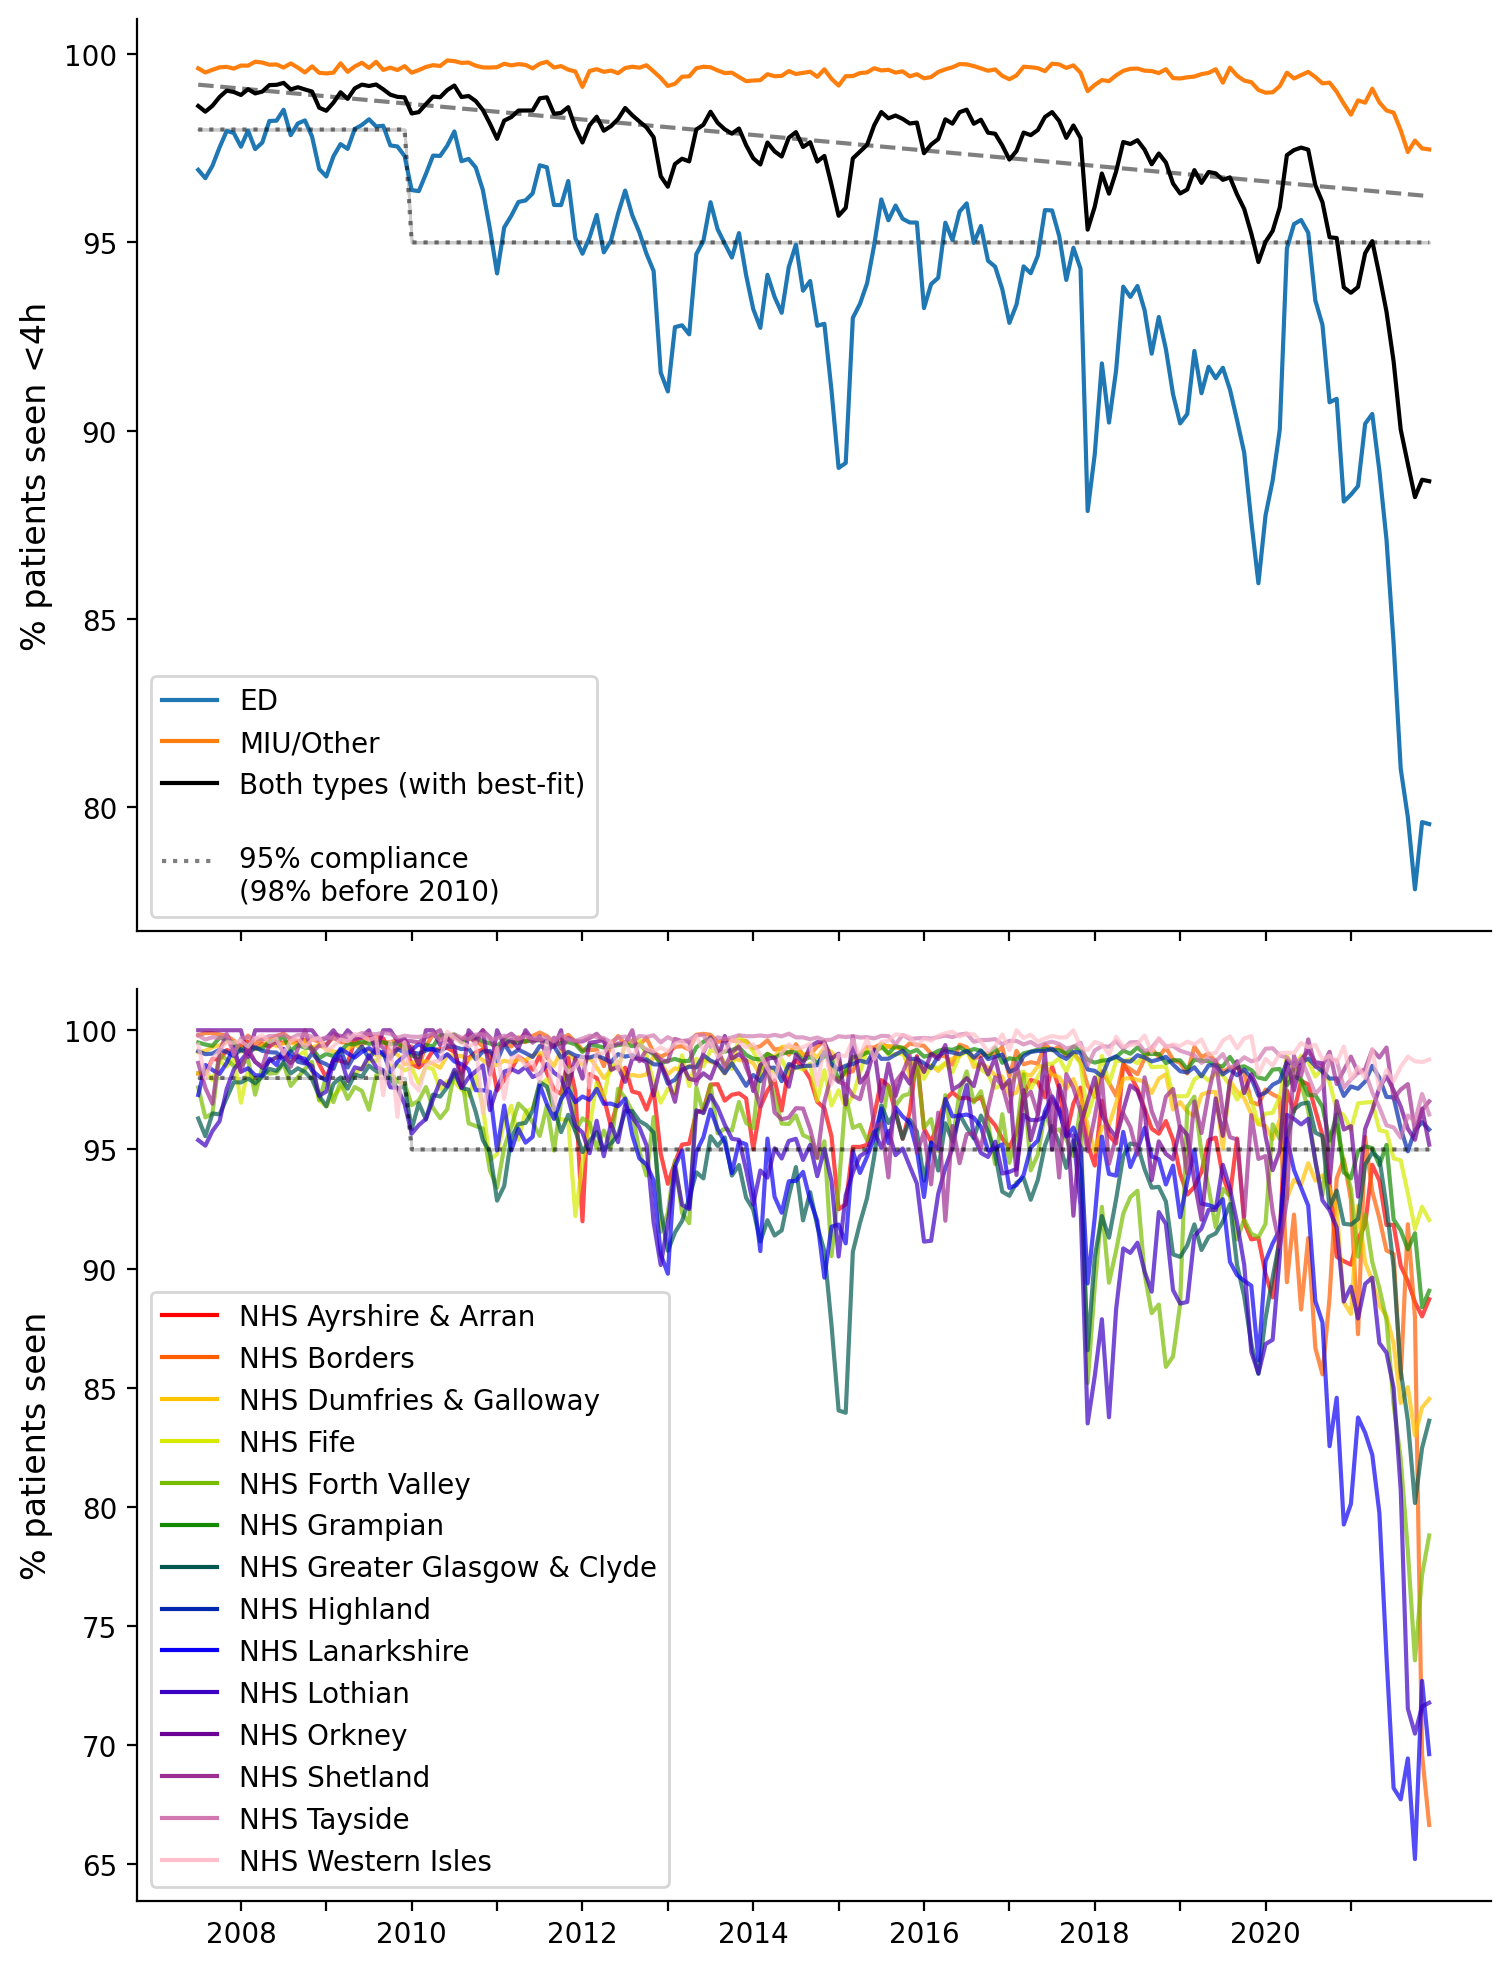
\includegraphics[width=\linewidth]{fig1.png}
    \caption{Monthly percentage of patients seen (admitted, transferred, or discharged) under 4h, by hospital type (top) and NHS board (bottom). Includes the 95\% compliance standard, as well as its past 98\% value.}
    \label{fig:fig1}
\end{wrapfigure}
Between 2007 and 2019, the average compliance has dropped by \textbf{0,205\%} each year ($R^2 = 0,589$), with Emergency Departments experiencing a much sharper decrease of \textbf{0,574\%} per year ($R^2 = 0,640$) compared to Minor Injury Units and others' approximate 0,024\% yearly decrease.\footnote{We say approximate since this is a very bad fit with $R^2 = 0,257$, implying large variance.} 
We confirm that the data does indeed have a very large heteroscedastic variance from the compliance by NHS board plot (Figure \ref{fig:fig1}).


To better visualise the differences between each region, in Figure \ref{fig:fig2} we plotted the per-region mean monthly compliance rates in the years 2008/09 and 2018/19, as well as a percentage change in compliance per region over 10 years by creating an OLS model for compliance in each region. The best-fit line is only on data before March 2020 to remove the effects of the pandemic.

\begin{figure}[h]
    \centering
    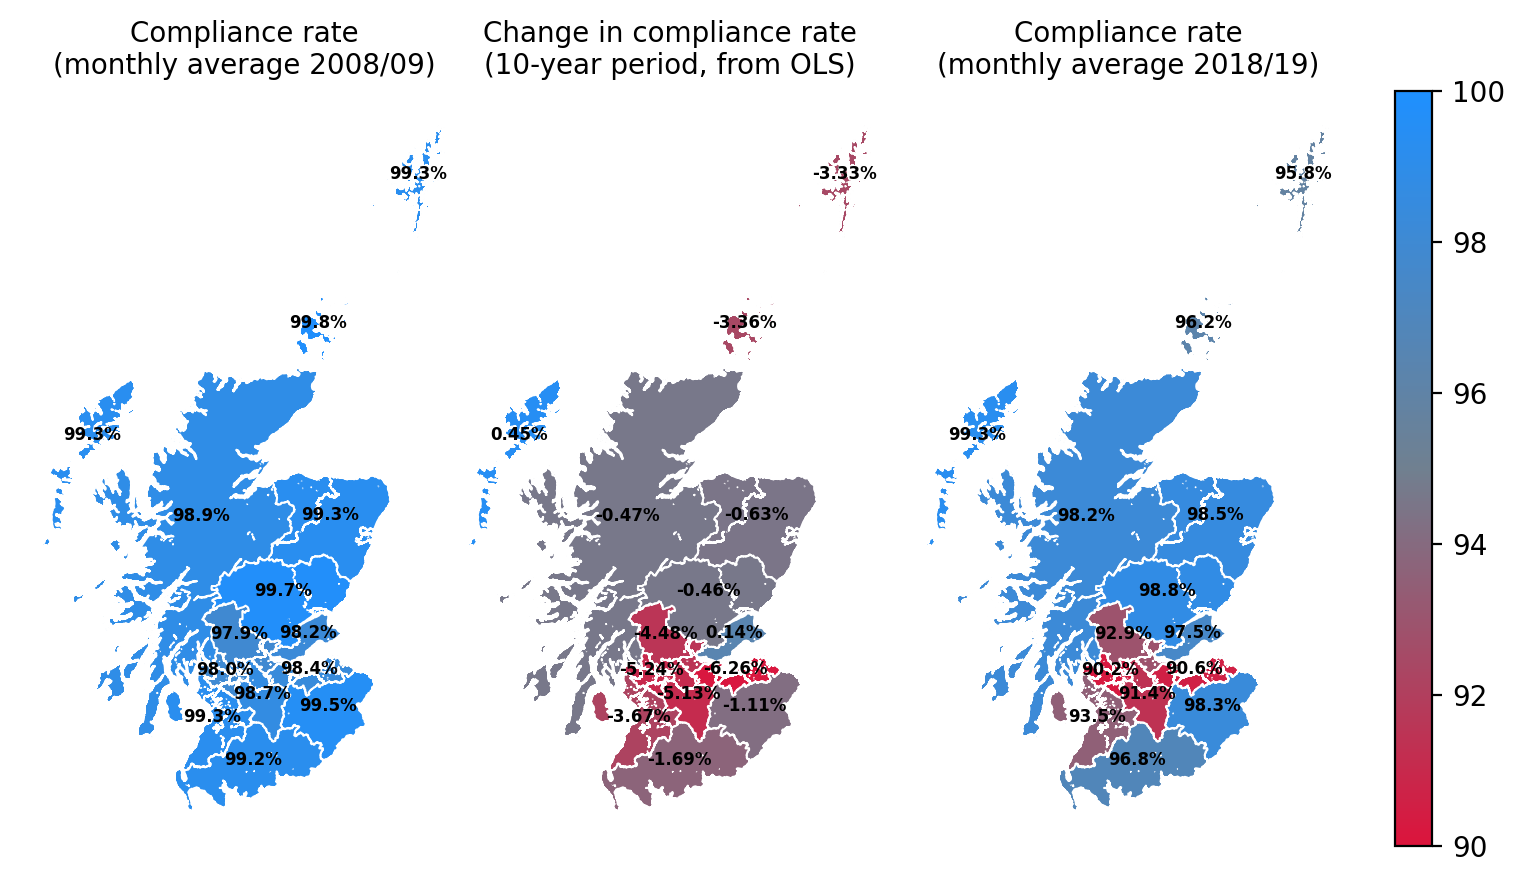
\includegraphics[width=\linewidth]{fig2.png}
    \caption{Average monthly percentage of patients seen (admitted, transferred, or discharged) under 4h per NHS board.}
    \label{fig:fig2}
\end{figure}

Here we notice that the regions that saw the largest decline in compliance like Lothian and Glasgow are the most populous (Figure \ref{fig:fig8}). To check that this is indeed the case, we plotted the total patients seen for each NHS board area (Figure \ref{fig:fig3}), and the pattern matches exactly to the regions that saw the largest decrease in compliance rates.

This leads us to our first hypothesis: there is an increase in the number of attendances to the A\&E, and the infrastructure is not able to keep up with this surge in demand. To confirm this, we calculated the cumulative fractional change in total patients, as well as the total population. 

\begin{wrapfigure}{r}{.4\linewidth}
    \centering
    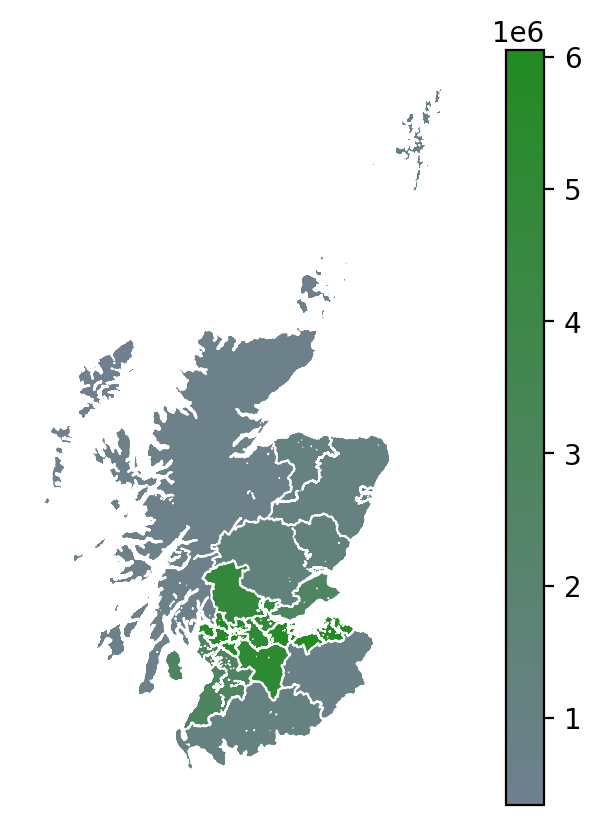
\includegraphics[width=\linewidth]{fig3.png}
    \caption{Total patients seen per NHS board between 2007 and 2022.}
    \label{fig:fig3}
    \vspace{-2em}
\end{wrapfigure}
We saw that the population increased by 0,245\% per year ($R^2 = 0,951$) whereas the total patients increased by 1,508\% per year ($R^2 = 0,894$). When we plot this in Figure \ref{fig:fig4} against the decreasing compliance rate, we can see that the increase in total patients is (not necessarily causally) correlated with the decrease in compliance. 

One possible explanation is that more people are attending the A\&E with less serious matters. We once again create OLS models for pre-pandemic data and create the plot, and see in Figure \ref{fig:fig4} that the amount of people staying in hospitals stays approximately constant (-0,17\% annually, $R^2 = 0,039$),
\begin{figure}[h]
    \centering
    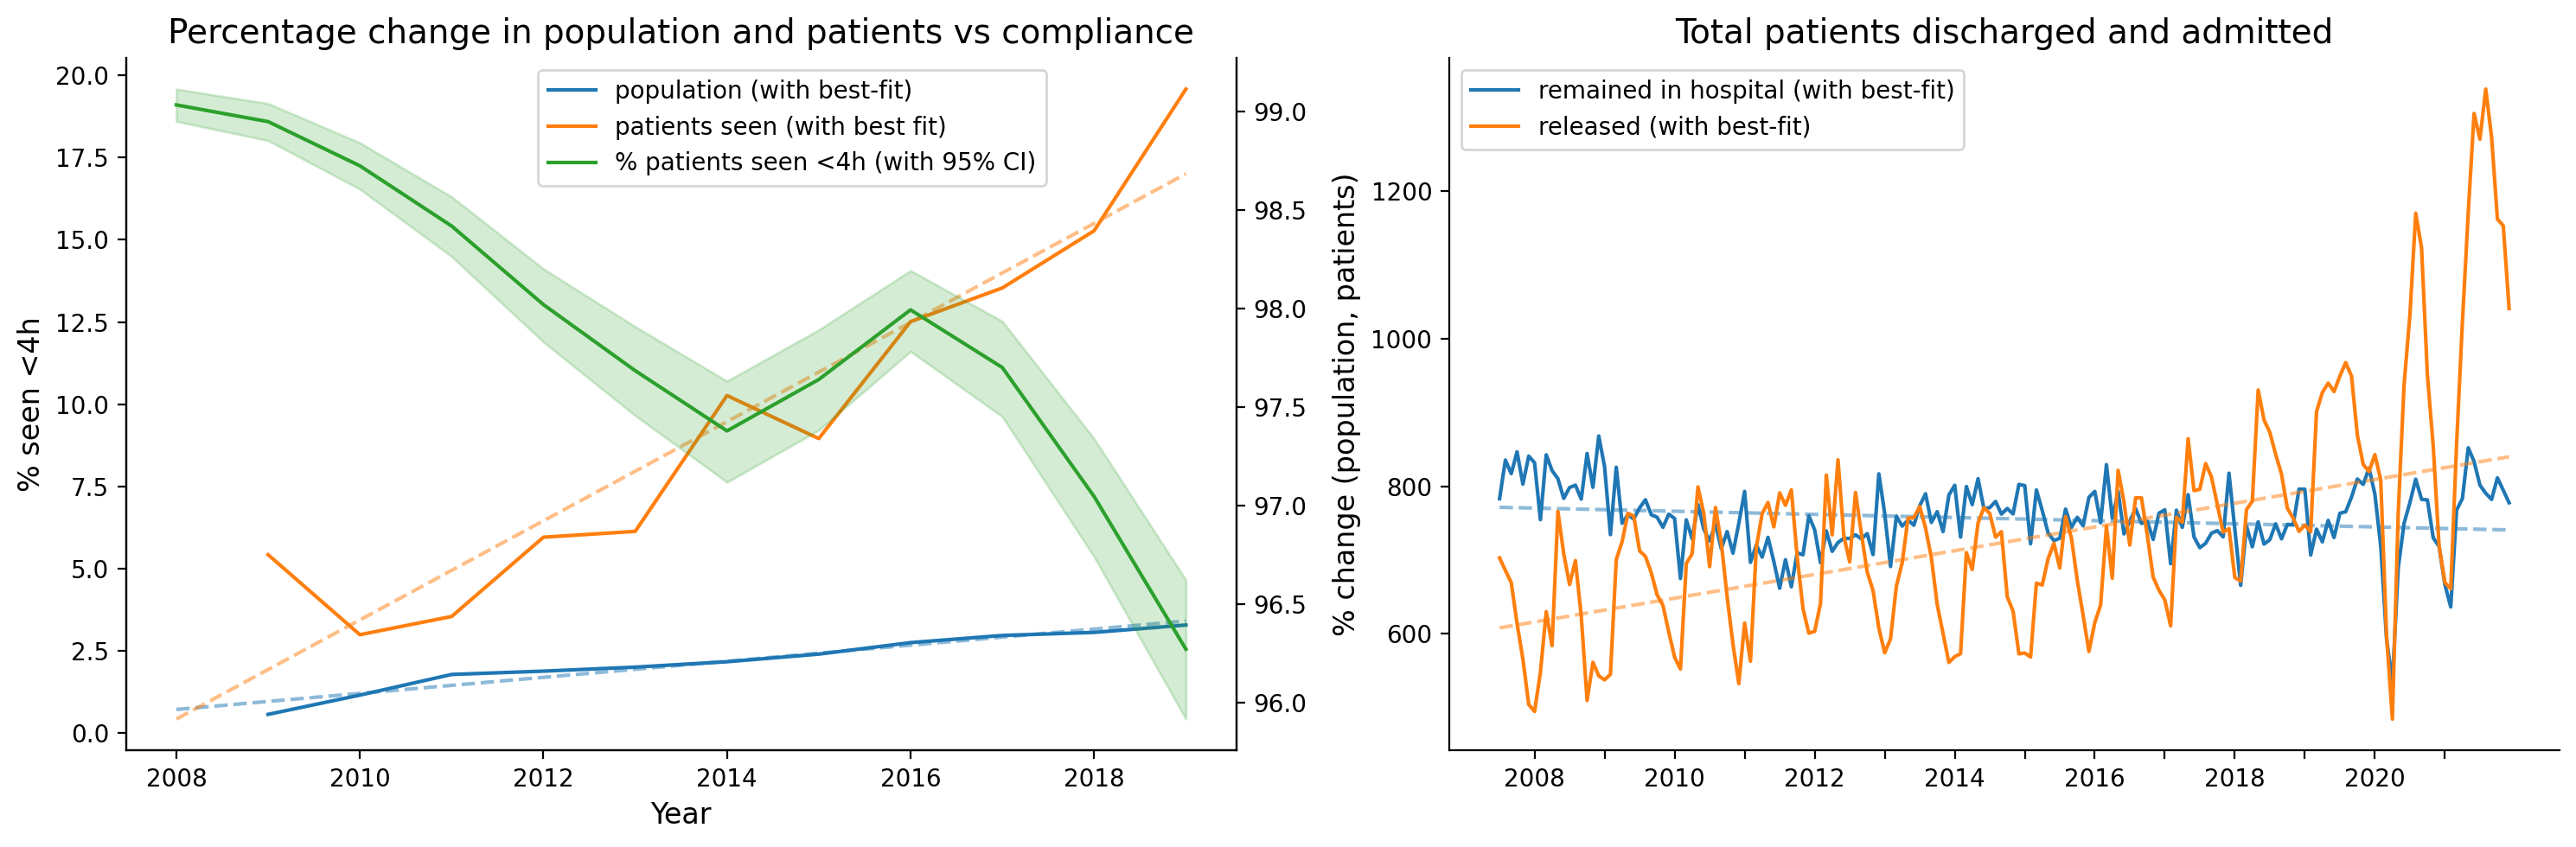
\includegraphics[width=\linewidth]{fig4.png}
    \caption{\textbf{Left:} Change in population, total patients, and compliance. Compliance 95\% CI calculated using $10^5$ bootstrap runs. \textbf{Right:} Total patients admitted and discharged from hospitals. \textbf{Note:} Best fits calculated with data before March 2020.}
    \label{fig:fig4}
\end{figure}
whereas the amount of people being discharged from the hospitals has seen an annual rise of 1,34\% ($R^2 = 0,334$). One possible explanation for this phenomenon is that the general practitioner (GP) infrastructure is lacking, and people are less likely to go to their GP with semi-urgent matters since they cannot get an appointment in time. Another possible explanation is the general ageing of the population which leads to increased health fragility and therefore an increase in A\&E visits.

Another way we can explore whether regions with large populations like Lothian and Glasgow are indeed the most problematic compliance-wise is to look at the hospital size. In Figure \ref{fig:fig5} we have plotted the total patients (we assume total patients to be proportional to hospital size) versus the number of patients seen under 4 hours. 
\begin{figure}[h]
    \centering
    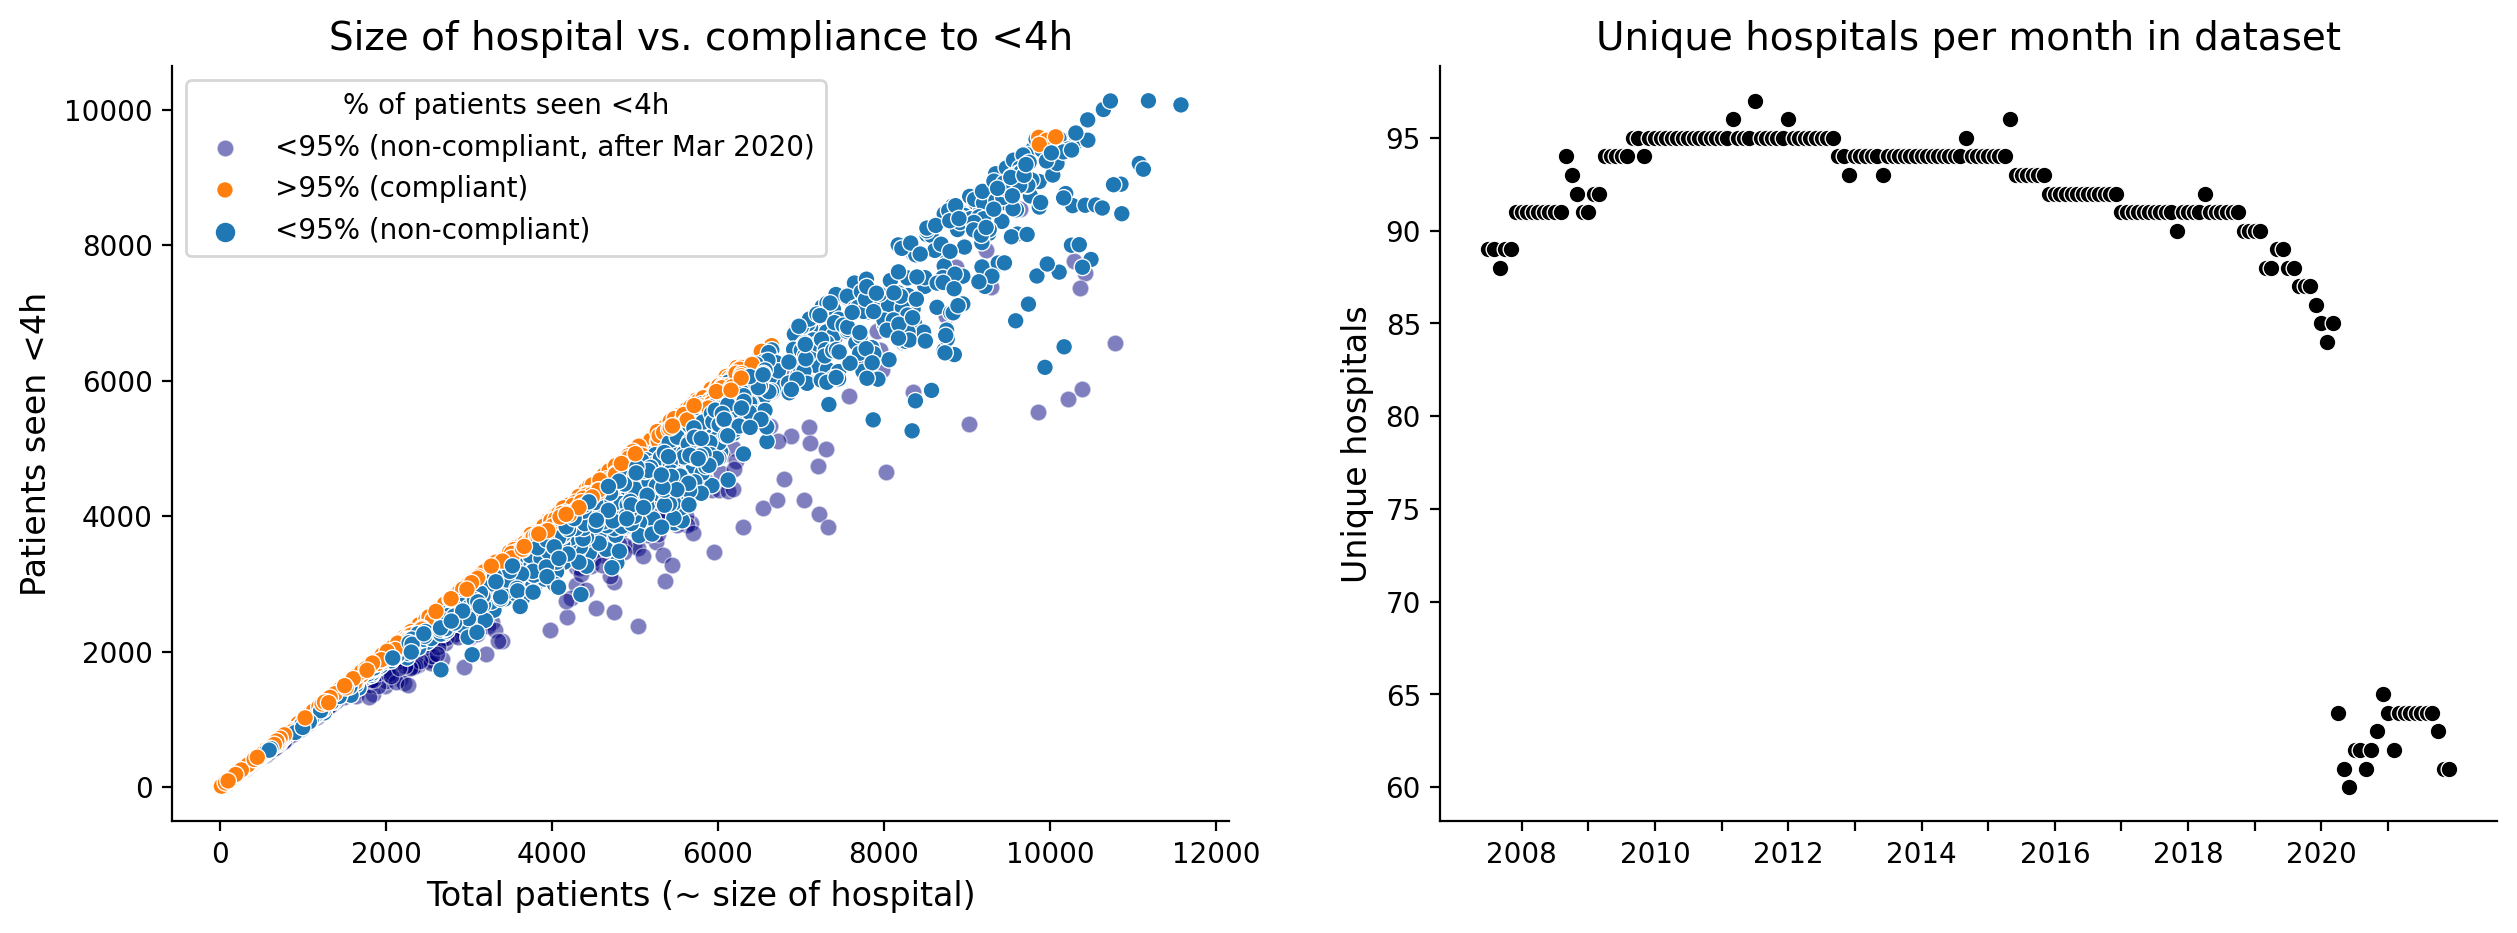
\includegraphics[width=\linewidth]{fig5.png}
    \caption{\textbf{Left:} Total patients vs patients seen within 4 hours. \textbf{Right:} Number of hospitals in the data set.}
    \label{fig:fig5}
\end{figure}
We can clearly see that as the total number of patients increases, compliance decreases, suggesting that hospital size does not scale proportionally to population needs, making wait times longer. However, note that the number of hospitals in the data set has not remained constant and the number of reporting hospitals decreased by $\sim$30\% during the COVID-19 pandemic.

Another avenue of exploration of the four-hour standard is to look at the seasonality of compliance trends. In Figure \ref{fig:fig6} we can see that the highest compliance occurs during the summer. This is interesting, since the summer months also see an influx of patients. The best explanation we have for this trend is that the nature of the visits changes based on the season. We hypothesise that during the summer months more young people attend with minor injuries, whereas during the winter the attendances include more elderly patients, since this is when diseases like the flu are more prevalent.
\begin{figure}[h]
    \centering
    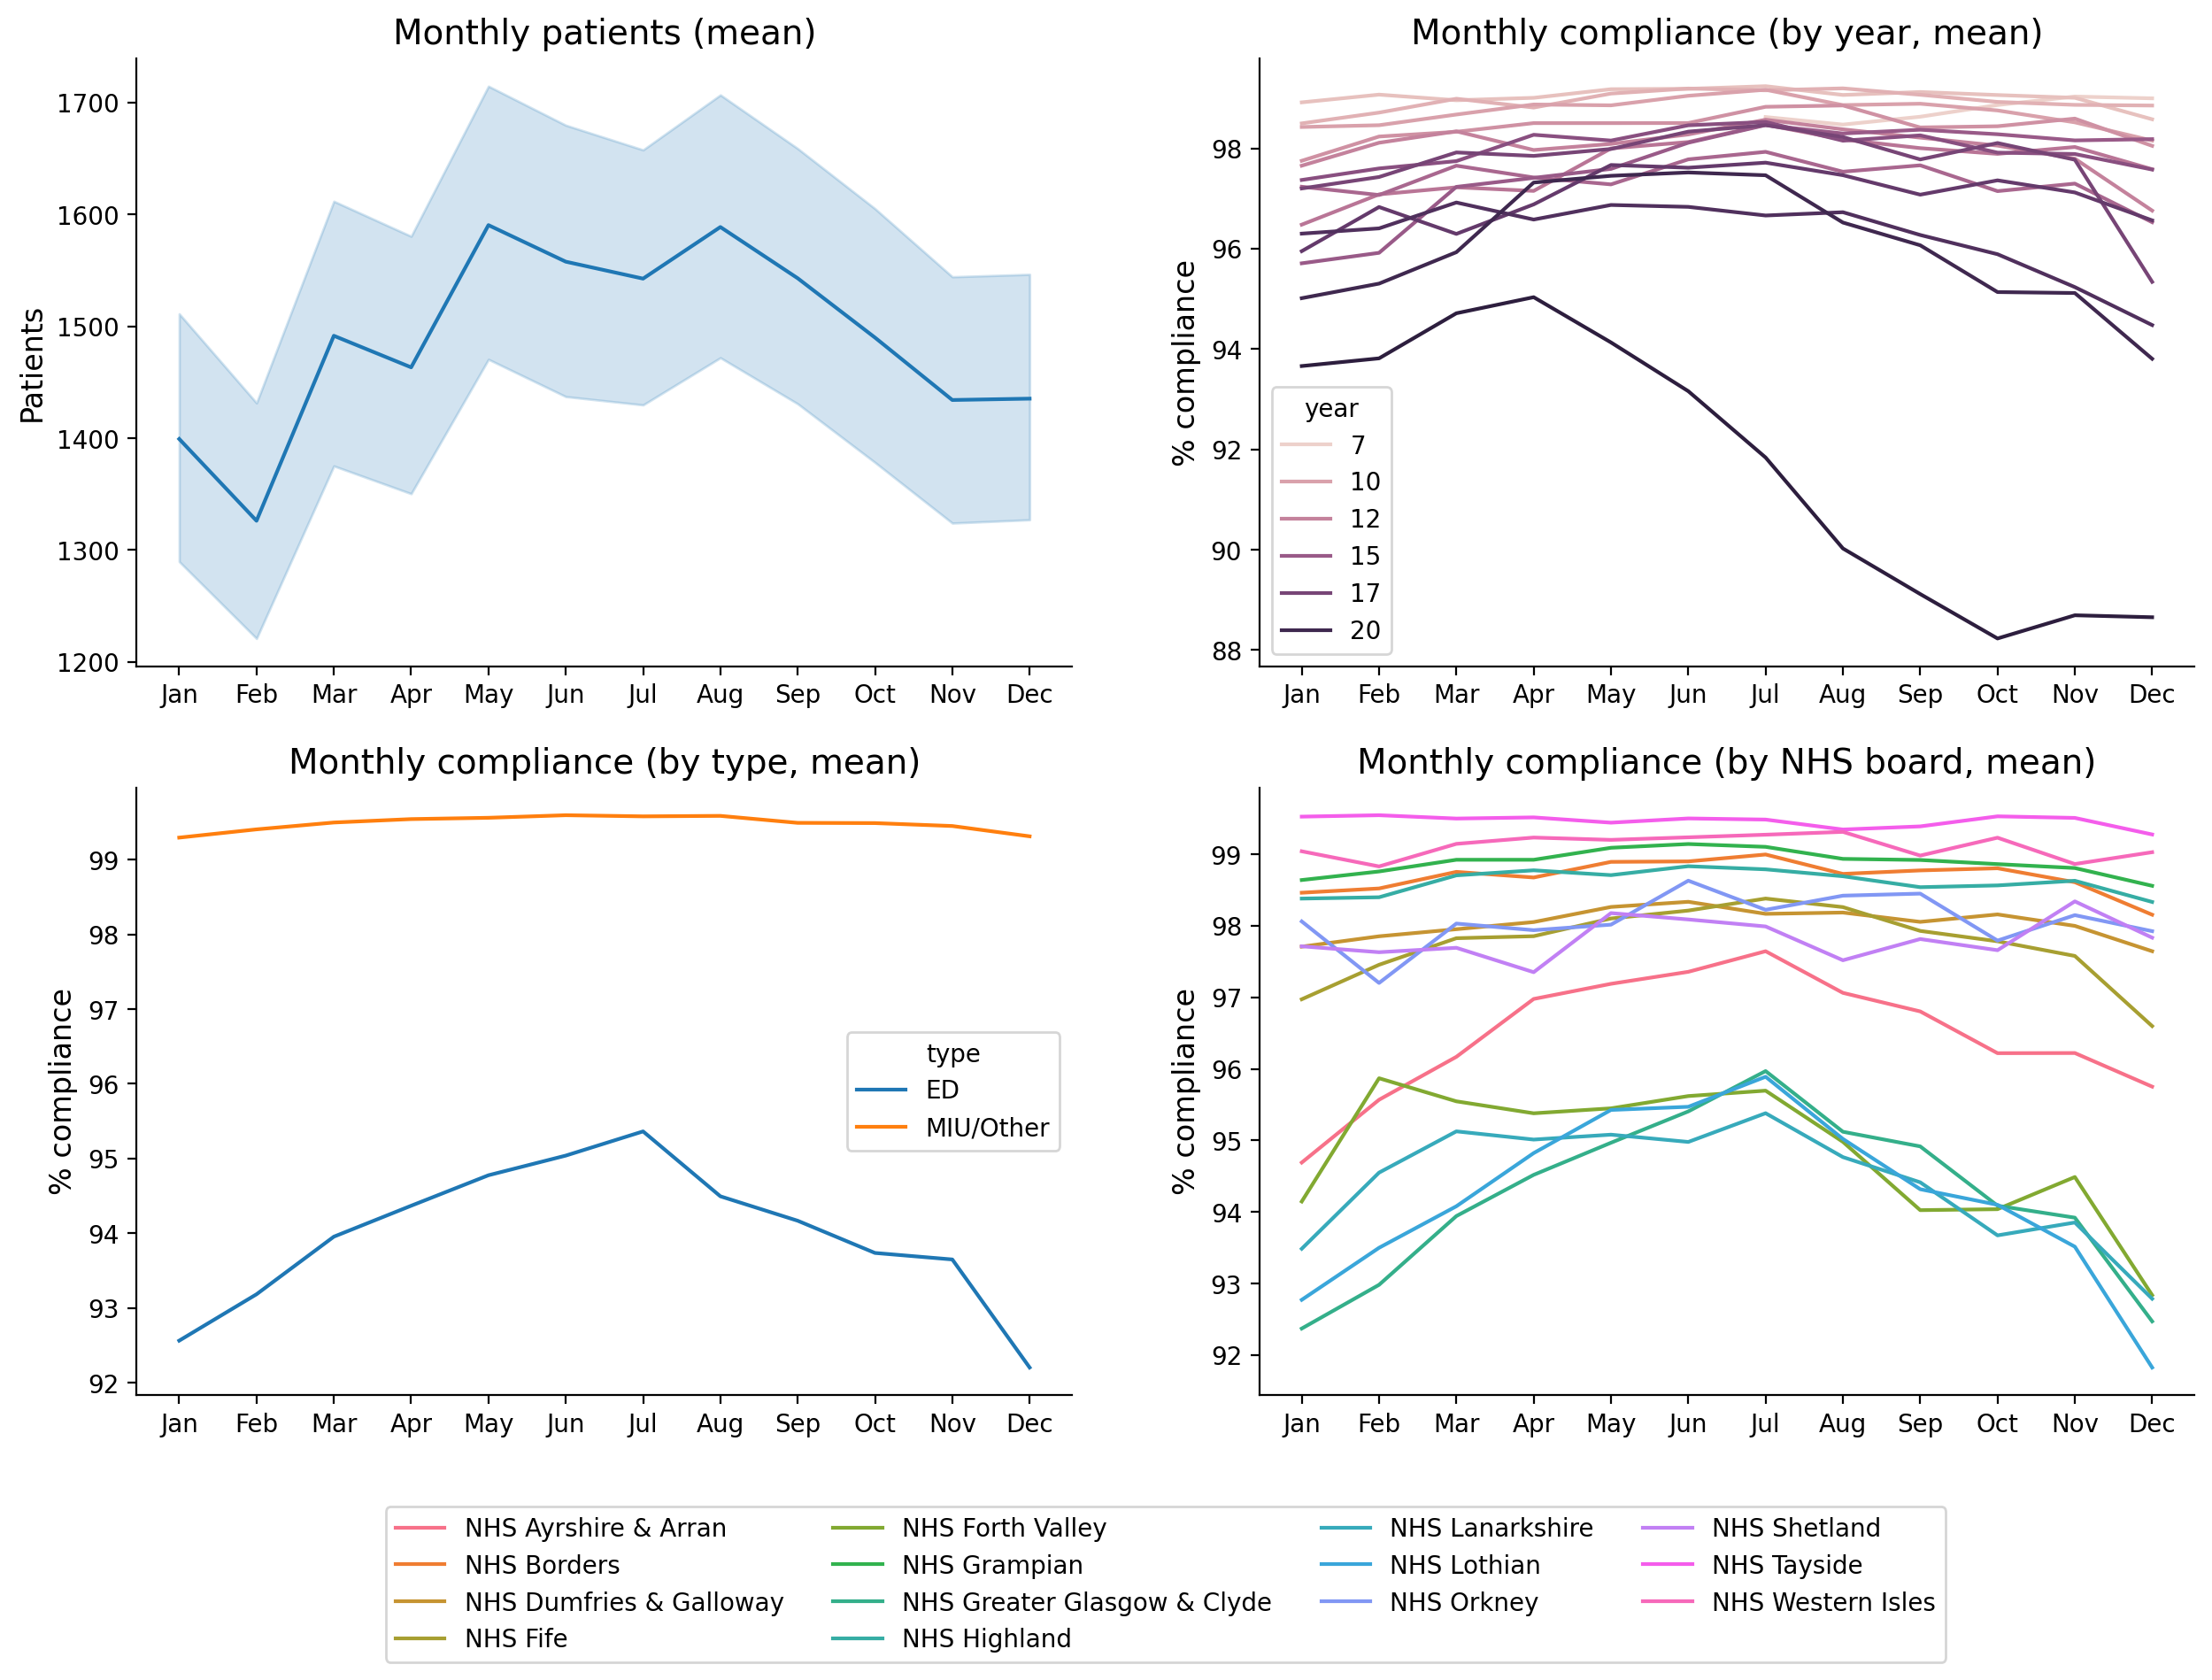
\includegraphics[width=\linewidth]{fig6.png}
    \caption{Seasonal graphs. Mean monthly patients shows 95\% spread.}
    \label{fig:fig6}
\end{figure}

\begin{wrapfigure}{r}{0.5\linewidth}
    \centering
    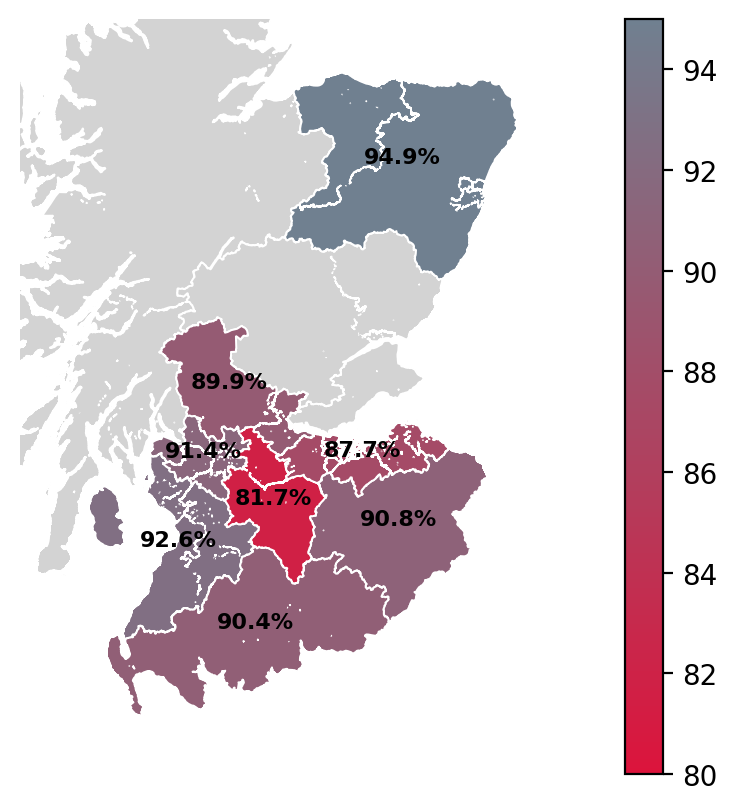
\includegraphics[width=\linewidth]{fig7.png}
    \caption{Mean compliance rate for non-compliant NHS boards (compliance averaged between Mar 2020 and Dec 2021).}
    \label{fig:fig7}
\end{wrapfigure}
Lastly, we briefly look at how the COVID-19 pandemic has impacted the compliance rates. In Figures \ref{fig:fig1} and \ref{fig:fig5} we see that the compliance rates have plummeted since the pandemic began. 
However, when we look at the compliance rates per NHS board, some of the boards have still managed to maintain an above 95\% compliance rate. We therefore calculated the average compliance rate between March 2020 and December 2021, and plotted only those boards that were not compliant in Figure \ref{fig:fig7}. All the other NHS boards have managed to maintain an average compliance of over 95\%. Here, we clearly see that the pandemic has had the largest impact on the most populous regions.
    
\section{Discussion and conclusions}

\begin{wrapfigure}{r}{0.45\linewidth}
    \vspace{-6em}
    \centering
    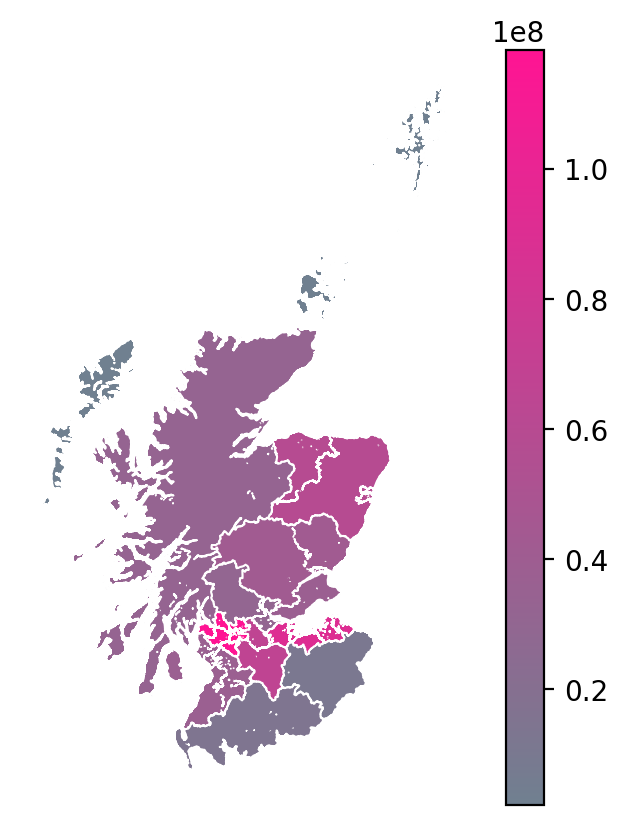
\includegraphics[width=\linewidth]{fig8.png}
    \caption{Population per NHS board (2021).}
    \label{fig:fig8}
    \vspace{-2em}
\end{wrapfigure}
In summary, we have seen that the compliance rates have been on a decline, with more populous regions seeing the largest downturn (NHS board populations plotted in Figure \ref{fig:fig8}). We have also observed that Emergency Departments (EDs) have a much worse compliance rate than Minor Injury Units (MIUs) and other hospital centres. Furthermore, we have shown that as the total patient number grows (approximately equal to a larger size of hospital) we see a sharp decline in the compliance rate (Figure \ref{fig:fig5}).

We have also found that the change in compliance is correlated with an increase in the total patients, which is much higher than the increase in population. We have speculated that this might be due to a lacking GP infrastructure, as well as a generally ageing population.

Last, we have looked at how the COVID-19 pandemic has impacted the compliance rates, and linked the observed effects with faults in the healthcare infrastructure we have observed by analysing the pre-pandemic data.

\subsection{Limitations of the analysis}
The data itself presented some inconsistencies which led our results to be less than accurate. Said inconsistencies arise from the fact that the data is submitted by hospital staff which for example can give different definitions to the \code{outcome} column. For example, we noticed that certain hospitals only presented three different outcomes (discharged to residence, discharged to other, or admitted to a hospital) while others made much more ample use of the discharge to unknown category.

Moreover, as we can see from Figure \ref{fig:fig5}, the number of hospitals submitting data is not consistent and has decreased significantly since the beginning of the COVID-19 pandemic, meaning that the pandemic evaluation may be skewed further. Last, we have not done any significance or scaling of factors to account for the fact that larger hospitals may be skewing the means.

Despite not being able to use many statistical methods since we were mainly focusing on description, rather than prediction, we believe that have have created powerful visualisations with the geographical plots that offer an new viewpoint on the NHS 4-hour standard data. We have also managed to obtain numerical estimates for the change of our values with OLS (ordinary least squares linear regression). The type and application of regressions could be improved to obtain a better $R^2$ value, but for extracting trends rather than interpolation we deemed OLS as sufficient.

\subsection{Comparison with related work}

Our general observation of declining compliance matches that of the Nuffield Trust and the King's Fund.\cite{the_nuffield_trust_2022}\cite{the_kings_fund_2020} In particular, our work is in agreement with the King's Fund analysis of seasonality which shows a clear drop in compliance over the winter, and with its analysis of how wait time relates to outcome, although neither of these phenomena are given an explanation in said publication. 

\subsection{Possible improvements and extensions} 

If a database that allows for this exists, it would be interesting to compare wait time with the resulting outcome. It was not possible to do this with the provided data set as the data was grouped by month, year and hospital and so we could not extrapolate which outcomes were related to which wait times.

A further extension that would be interesting to develop is an analysis of post-COVID trends (when such a time comes) to see if the pre-pandemic trends return as the were or if they have been skewed positively by the pandemic in the long run.

\newpage
\addcontentsline{toc}{section}{References}

\thispagestyle{empty}
\def\UrlBreaks{\do\/\do-}
\footnotesize{
    \bibliography{references.bib}
}
\end{document}